\chapter{Introduction}
\section{Motivation}
Without cell adhesion no complex life would exist \cite{REF}.
This is a well known and long existing statement in the biology. It describes that if different cells would not stick to each other the only living things would be cells. 
In humans, organs are made of severall cells. This is also the case for the urothelium. For the urothelium it is necessary that the cells stick to each other. Otherwise the functions of the urothelium could not be executed and also it would not be able to growth.% If bladder cancer occurs the urothelium also can not function in the way it should do. 

There are two types of tumors. One is the benign and the other one is the malignant tumor \cite{Poplawski2009}. The benign tumor is self limited. Thus, it does not invade surrounding tissues as well as it does not spread into other body parts \cite{Poplawski2009}. The malignant tumor on the other hand is not limited in its growth and is able to invade other body parts \cite{Poplawski2009}. 
Since bladder cancer is one of the most common cancer types among men it is important to understand how and why the cancer is able to growth. Bladder cancer starts to growth in the urothelium. With the growth and spread the structure of cells sticking together is changed. In this case, the urothelium is not able to completely do its tasks. In order to understand the urothelium and how and when bladder cancer appears observations of this organ are necessary. 

To understand the functionality of organs observation is necessary. For the urothelium this is already done, as there are a lot of different in vitro experiments about the methodology of the urothlium. After the observation of organs is complete, we are able to predict how the organ will react to different situations. To verify these predictions we need to simulate the behavior of the organ. A simulation is in generell an illustration of the reality, but it can also be used to change reality in a for the research specific way to get more knowledge of this organ.

A simulation should always be a simple as possible but also not to simple. Otherwise the simulation does not displays the reality. In the moduro project there is a 2D simulation of 16 different models of the urothelium. After all them were simulated the result is that the models are more realistic and others are less. The target with these models is to predict when bladder cancer occurs.

Because a cell is a three dimensional organism, a 2D simulation of the urothelium might not give as many aspects as a 3D simultion could do. The aim of this bachelor thesis is to create a 3D simulation of these 16 different models. With this 3D simulation new insights of the urothelium and how bladder cancer occurs will be received. 

\section{Background}
\subsection{Biology of the Urothelium}
Bladder cancer is the 4th most common cancer type in men regarding to everydayhealth.com \cite{EveryDayHealth.com}, where every 36st out of 100.000 men gets it. Bladder cancer usually starts with some cells in the bladder, which growth uncontrolled. From these cells, the tumor can spread further into surrounding areas \cite{Cancer.org}. The most common bladder cancer type is the urothelial carcinoma \cite{Cancer.org}. An illustration of how bladder cancer evolves is displayed in figure \ref{img:physiology_urothelium} at page \pageref{img:physiology_urothelium}.

The bladder is located in the lower urinary tract and consist of several parts, where urothelium coats the bladder \cite{Lazzeri2006}. More specifically, it covers the bladder from the renal pelvis to the proximal urethra \cite{Yamany2014, Birder2005} 

Two important tasks of the bladder are the storage and release of urine. To do so the bladder will extend, during the storage, and then shrink again \cite{Karl-ErikAndersson2004}. One task of the urothelium is to form a distensible barrier \cite{Apodaca2004, Lazzeri2006, PuneetKhandelwal2009, Lewis2000, WRCross2005}, which prevents unregulated exchange of ions, solutes, and toxic metabolites between the bladder and the blood \cite{Apodaca2004, Lazzeri2006, PuneetKhandelwal2009, Lewis2000}. That the urothelium ensures its barrier function, it has to growth and downsize its size. This is done by the largest cells of the urothelium – the umbrella cells. Because the umbrella cells are in direct contact with the bladder, it is their task to change size and form during the growth and shrink process of the bladder. Birder described the urothelium as “… a responsive structure capable of detecting physiological and chemical stimuli and releasing a number of signaling mole-cules.” \cite{Birder2005}. Another task of the urothelium is to control the movement and passage of macromolecules, ions, water, toxic metabolites and solutes \cite{Apodaca2004, PuneetKhandelwal2009}. If the urothelium is damaged, it rapidly generates new cells, to ensure full functionality \cite{Apodaca2004, Yamany2014, PuneetKhandelwal2009}. In the research there are assumptions, that the quick regeneration is done by a lot of mitosis, i.e. cell division.

To receive a better overview the different cell types are explained in the following paragraph. In figure \ref{img:physiology_urothelium} at page \pageref{img:physiology_urothelium} a simplified illustration of the urothelium with its different cell types and cell layers is provided. \newline
The umbrella cells, also called superficial cells, they are connected directly with the bladder and have an average diameter of 25 up to \SI{250}{\micro\metre} \cite{Yamany2014, PuneetKhandelwal2009}. 

Below these cells the intermediate cells are located. With an average diameter of 10 up to \SI{20}{\micro\metre} \cite{Yamany2014, PuneetKhandelwal2009}, they are a far bit smaller then the umbrella cells. The middle layer of the urothelium can consist of several own layers, i.e. there can be several layers in the layer of the intermediate cells. 

The smallest and the most common cells in the urothelium are the basal and stem cells. Those cells have a diameter of up to \SI{10}{\micro\metre} \cite{Lazzeri2006, PuneetKhandelwal2009}. 

The urothelium has several layers. In the first layer, there are the basal and stem cells. Above them, there are several layers of intermediate cells. On top of the epithelium, i.e. a membranous tissue which consists of one or several layers1, there is one layer of umbrella cells.

\begin{figure}
	\center
	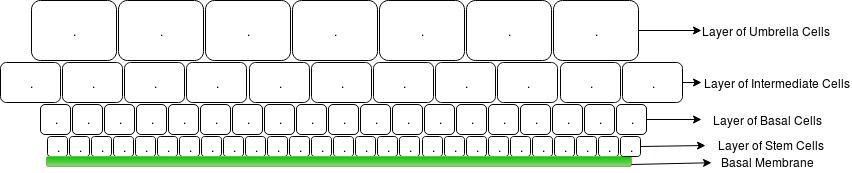
\includegraphics[scale=0.6]{figures/Urothelium.png}
	\caption{Simplified physiology of the urothelium}
	\label{img:physiology_urothelium}
\end{figure}

\subsection{Glazier Graner Hogeweg Model} \label{subsec:Intro_GGH}
Since there are several formulas and models developed from Glazier and Graner, this subsection briefly describes these models and formulars.\newline
\ac{GGH} models are widely used in biological simulations, since it provides a good flexibility, extensibility and it is easy to use \cite{Glazier2007}. 
Glazier and Graner developed their model as an extension of the large-q Potts model, which itself is an extension of the Ising Model, and called it first the \ac{EPM}. Nowadays, this model is called \ac{CPM} \cite{Glazier2007, Graner1992, Glazier1993}.
Glazier and Graner extended their \ac{CPM} in a way that also volume constraints are considered for the hamiltonian, see following form:
\begin{equation}
\begin{split}
\mathcal{H}_{CPM} & = \sum_{\vec{i},\vec{j}}^{ }J(\tau(\sigma(\vec{i})),(\tau(\sigma(\vec{j})))(1-\delta(\sigma(\vec{i}),(\sigma(\vec{j}))) \\
		 & + \sum_{\sigma}^{}{\lambda_{vol}(\tau)v(\sigma)-V_{target}(\tau(\sigma)))^2}
\end{split}
\end{equation}
This hamiltonian, describes first the adhesion energy between different cell types. Therefor, every cell has a specific cell type $\tau(\sigma)$ \cite{Glazier1993, Graner1992}. Each cell is placed onto a lattice with a spin $(\sigma(\vec{i}, \vec{i})$ for every given dimension \cite{Glazier1993, Graner1992, Glazier2007}. The adhesion energy between cells is only considered if the kroenecker delta is 0. Thus, the surface energy between cells is considered if $\delta(\sigma, \sigma') = 0$ \cite{Glazier1993, Graner1992, Stott1999, Glazier2007, Chen2007, Cickovski2005}. Second, the volume of each cell is now considered and the user is allowed to add a multiplier to the hamiltonian, which is done by the multiplier $\lambda_{vol}$.

Together with Hogeweg they further develop their created extension of the \ac{CPM}. The further developed model is today called \ac{GGH} model. The main extension was that the user of \ac{GGH} model is now able to add surface area constraints \cite{Graner1992, Glazier1993, Glazier2007} as well as to use a negative boundary energy \cite{Glazier2007}. With the surface are constraint the formula for the \ac{GGH} model is: 
\begin{equation}
\begin{split}
\mathcal{H}_{GGH} & = \sum_{\vec{i},\vec{j}}^{ }J(\tau(\sigma(\vec{i})),(\tau(\sigma(\vec{j})))(1-\delta(\sigma(\vec{i}),(\sigma(\vec{j}))) \\
		 & + \sum_{\sigma}^{}{\lambda_{vol}(\tau)v(\sigma)-V_{target}(\tau(\sigma)))^2} \\
		 & + \sum_{\sigma}^{}{\lambda_{sur}(\tau)s(\sigma)-S_{target}(\tau(\sigma)))^2}
\end{split}
\end{equation}
The new model also allows the user to model (a): cell growth and proliferation (b): mitosis, i.e. cell division (c): fields, forces and diffusion and (d): chemotaxis and haptotaxis \cite{Glazier2007}.

Glazier et. al. describe their model as: 
\begin{quote}
GGH models define biological structure consisting of the configuration of a set of \textit{generalized cells}, each represented on a \textit{cell lattice} as a domain of latitice sites sharing the same cell index [...], a set of \textit{internal cell states} for each cell [...], and a set of \textit{auxiliary fields} ...” \cite{Glazier2007}.
\end{quote}

The \ac{GGH} model has the advantage that “Initial conditions emulating a particular biological configuration rather than random initial conditions.” \cite{Glazier2007} and it has now biologically motivated properties instead of physically motivated properties \cite{Glazier2007}. 


\subsection{CompuCell3D}
\ac{CC3D} is an open-source program, which provides a simulation environment for multi- or single-cell-based modeling of tissues, organs and organisms \cite{CC3D.org}. To do so, \ac{CC3D} uses the \ac{CPM} in its simulation \cite{CC3D.org}, which describes cell and \ac{ECM} behavior \cite{Izaguirre2004}. 
CC3D provides the possibility to create scripts for the simulation, e.g. cell growth, mitosis, apoptosis or necrosis scripts, in python, C++ or in their own CC3DM, which is their own Markup Language. With such scripts CC3D allows the user to modify the behavior of the simulation for a specific purpose.
CC3D uses the \ac{GGH} approach, explained in section \ref{subsec:Intro_GGH} at page \pageref{subsec:Intro_GGH}. It allows the user to choose between several cell-lattice types, i.e. a presentation of the pixels of a cell at a specific position in the simulation field (see picture XY). By default, it uses a square-lattice of single pixels for each dimension. There is also the possibility to use a hexagonal-lattice, where the pixels would be hexagons in two dimensions, or rhombic dodecahedrons in three dimensions.
Since the core of a \ac{GGH} simulation is the effective energy \cite{IntroCC3D}, \ac{CC3D} tries to minimize this effective energy every \ac{MCS}, i.e. a calculation step in the simulation. The basic form for the effective energy is:
\begin{equation}
\mathcal{H}_{boundary} = \sum_{\vec{i},\vec{j}}^{ }{J(\tau(\sigma(\vec{i})),(\tau(\sigma(\vec{j})))(1-\delta(\sigma(\vec{i}),(\sigma(\vec{j})))}
\end{equation}
There are several ways to extend this form, it is possible to add a volume or a surface constraint. During each \ac{MCS} an index-copy attempt takes place \cite{MaciejH.Swat2017}. I.e. a pixel is selected, and it will be tried to overwrite a randomly chosen pixel, next to the current pixel, in order to minimize the effective energy. The index copy attempt succeed and takes place only if this index copy attempt decreases the effective energy \cite{IntroCC3D}. Each \ac{MCS} the program tries to minimize the simulation, e.g. with index copy attempts. The user has the chance to use her/his specific script every \ac{MCS}, before the simulation starts or at the end of the simulation.


\section{Objective of the Bachelor Thesis}
The aim of this bachelor thesis is to create a 3D morphogenesis simulation of the urothelium using \ac{CC3D}. Since the simulation models and python program for a 2D simulation are given and the simulation is done by \ac{CC3D} the task is to modify the current application, of the 2D simulation, in a way that this program can be used for a 3D simulation of the different models. \newline
Therefore, some parts of the program have to be modified. Some functionalities has to be written completely new wheras for other functionalities it is enough to modify these. \newline
The result of this bachelor thesis will be presented with an of the 2D simulation realistic model. This model is choosen from the given models in the 2D simulation. The question how much more time the 3D simulation need than the 2D simulation will be covered in this thesis as well. If it is possible to provide a calculation of how much more effort a simulation in three dimensions need it will be included, otherwise an estimation of the more effort is presented.


\section{Outline}
In this chapter the knowledge to understand this bachelor thesis is provided. The next chapter provides the status at which the project was at the beginning of this bachelor thesis. Once the basic knowledge and the state of the art are explained, necessary modifications of the program are revealed. After these modifications are presented, the result of this bachelor thesis is shown. In the last section of this scientific work this thesis is discussed from different points of view and the conclusion out of this work is presented.